\chapter{Planificación e Avaliación de Custes}

A planificación e a avaliación de custes son de vital importancia nun proxecto destas 
características, pois aseguran que o proxecto de desenvolverá correctamente cumprindo con todas as
especificacións desexadas. Neste caso a realización do proxecto abarca dende comezos de febreiro de
2015 cando teñen lugar as primeiras reunións ate setembro de ese mesmo ano no que finaliza a 
execución desta aplicación e a elaboración da memoria co obxectivo de presentar o conxunto do 
traballo a mediados de setembro.

Como se explicou no capítulo referente á metodoloxía, o proxecto subdividirase nunha serie de 
iteracións de aproximadamente un mes de duración\footnote{As datas non son de un mes exacto xa que
se adaptaron estes períodos en función da carga lectiva e de outras variables de carácter persoal 
para cumprir así coa faceta incremental do proxecto, facendo que cada nova Release aportase unha
serie de características de interese.} e trinta horas de traballo aproximadamente\footnote{ 
A excepción do último sprint pertencente ao mes de Agosto, no que posuía dispoñibilidade a tempo
completo},
nas que se acometerán unha serie de 
funcionalidades concretas. Para o seguimento do avance do proxecto, o seu control e avaliación 
empregase a ferramenta YouTrack, que a parte de xestionar de forma áxil as tarefas a realizar, 
permite xerar informes de proxecto como os que se verán a continuación. A parte disto, por cada 
versión estable pódese atopar no repositorio de GitHub, unha Release co seu número de versión e o 
seu comentario asociado. As Releases pódense ver na seguinte lista:

\begin{itemize}
 \item \textbf{v0.1 - Cargar e Visualizar vídeos} (1 febreiro - 1 marzo) 
 \item \textbf{v0.2 - Subida e Conversión de vídeos} (1 marzo - 19 abril)
 \item \textbf{v0.3 - Xerar e mostrar deteccións básicas} (19 abril - 15 maio)
 \item \textbf{v0.4 - Arranxar bug's e mellorar a estratexia de probas} (15 maio - 11 xuño)
 \item \textbf{v0.5 - Traxectorias}  (11 xuño - 10 xulio)
 \item \textbf{v0.6 - Detección do comportamento anómalo} (10 xulio - 24 xulio)
 \item \textbf{v1.0 - Memoria e posta en produción} (24 xulio - 30 agosto)
\end{itemize}

A primeira iteración do proxecto estivo principalmente centrada na formación sobre o framework
Django, xa que o fin primordial era o de crear unha primeira páxina web que permitise subir e 
visualizar vídeos. Tamén estivo centrada en coñecer de preto as posibilidades ofertadas pola
ferramenta GitHub para poder subir os avances realizados. Non se empregaba por tanto ningunha
ferramenta para o seguimento de incidencias ou a integración continua.

Durante a segunda e terceira iteración cando xa se dominaban tanto Django como GitHub, 
procedeuse á busca dunha ferramenta para este seguimento de incidencias. Nun comezo, empregouse
a propia ferramenta integrada en GitHub que permite un seguimento mínimo das tarefas e as metas
a alcanzar, e xa na terceira iteración optouse de forma definitiva por YouTrack, migrando os 
issue's acumulados en GitHub a esta nova plataforma máis completa. Durante este período tamén se
foi configurando Travis CI como servidor de integración continua, inda que a ampla diversidade
de linguaxes e tecnoloxías presentes no proxecto fixo que esta integración continua fallase 
eventualmente por motivos de configuración.


Na gráfica \ref{fig:fluxoAcumulado} podemos ver o fluxo acumulado de tarefas no cal se distinguen
as tarefas \textbf{abertas}, \textbf{en curso} e \textbf{solucionadas}. A gráfica amosa un fluxo 
crecente de tarefas solucionadas correspondentes ás tarefas realizadas en cada iteración e tamén 
unha serie de tarefas pendentes que corresponden as tarefas do Product Backlog que nunca chegaron
a entrar en ningún Sprint por falta de prioridade e que conformarán a meirande parte das liñas 
futuras do capítulo \ref{sec:linhasFuturas}.

\begin{figure}[htp]
\begin{center}
    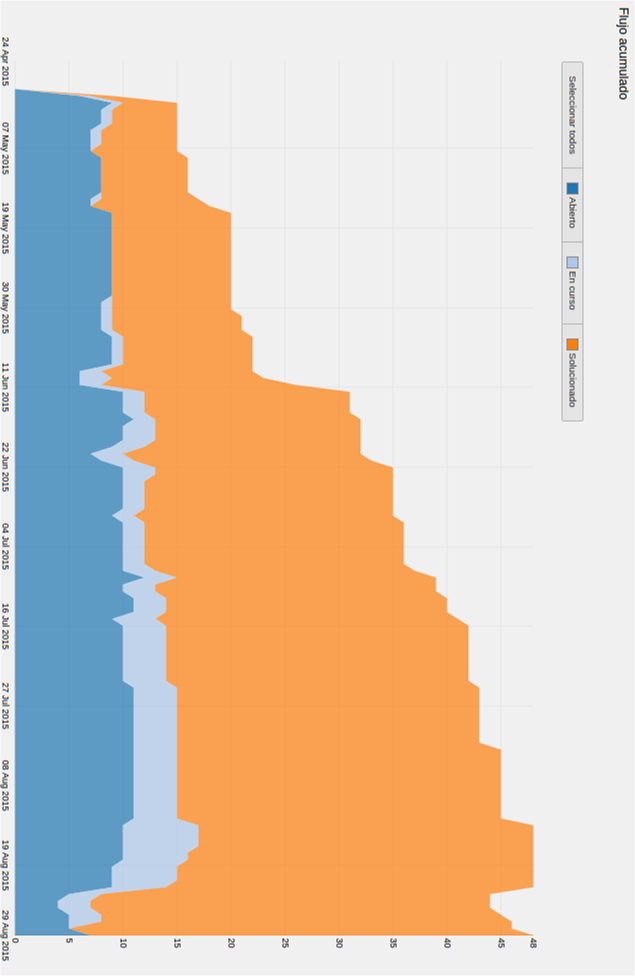
\includegraphics[scale=0.6]{figures/YouTrack/fluxoAcumulado.png}
    \caption{Gráfica do fluxo de tarefas acumulado ao longo do proxecto}
\label{fig:fluxoAcumulado}
\end{center}
\end{figure}

Por outra parte o gráfico de evolución do proxecto (figura \ref{fig:evolucionProxecto}) marcou 
durante o desenvolvemento dos sprints a liña idónea e por tanto a velocidade en relación ao ritmo
ideal. Nótese que a gráfica estima por número de tarefas e non por horas estimadas, isto 
explica as desviacións como as do mes de agosto, xa que ao dedicarse esta iteración practicamente á
memoria e ser a memoria unha única tarefa, a gráfica permanece estanca aínda que se sigan a sumar
horas de traballo de forma continua.

\begin{figure}[htp]
\begin{center}
    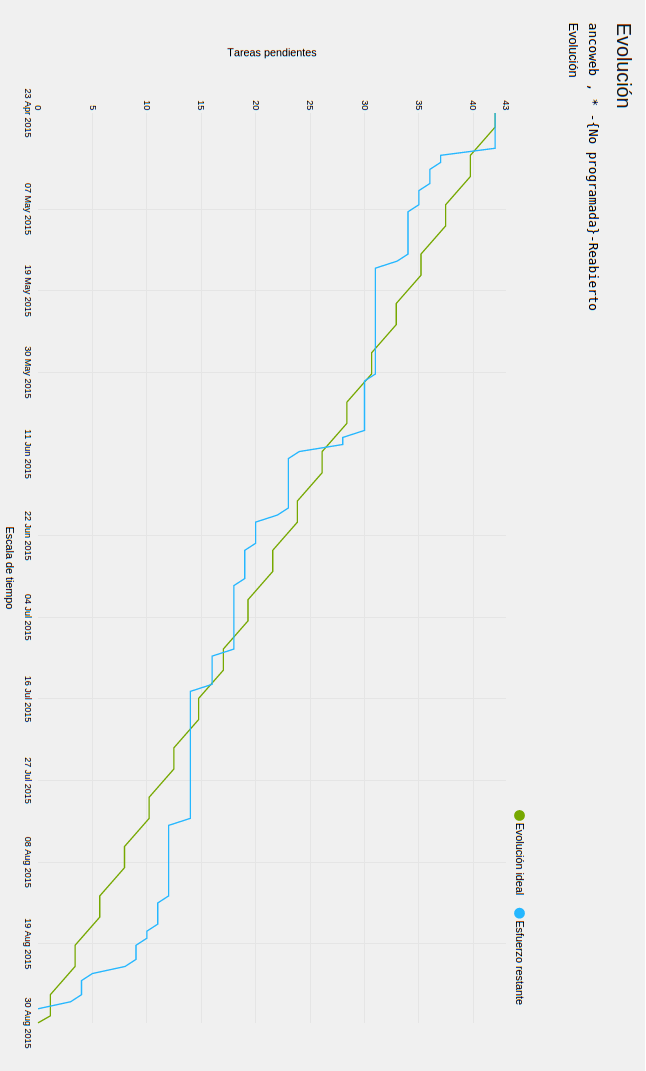
\includegraphics[scale=0.6]{figures/YouTrack/evolucionProxecto.png}
    \caption{Gráfica da evolución do proxecto}
\label{fig:evolucionProxecto}
\end{center}
\end{figure}



\begin{figure}[htp]
\begin{center}
    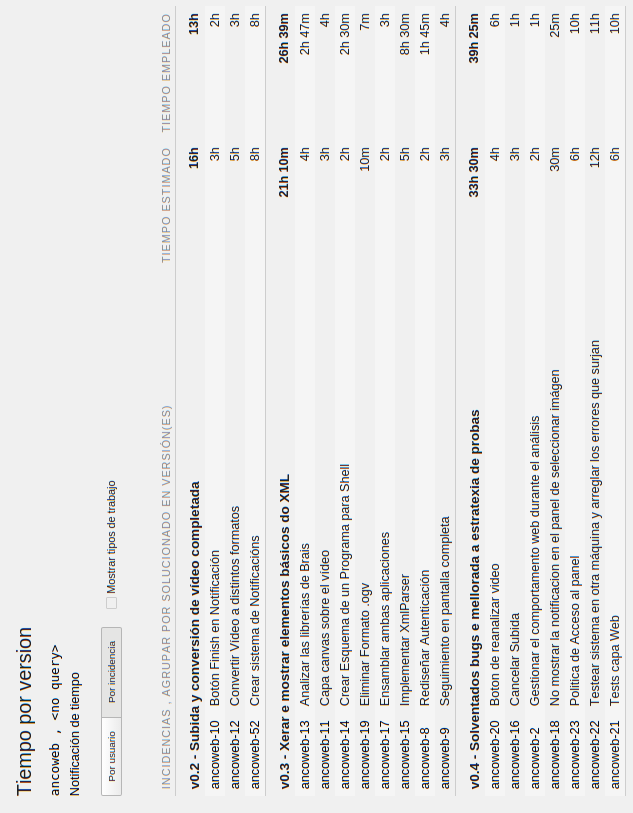
\includegraphics[scale=0.7]{figures/YouTrack/taboaHoras2_1.png}
    \caption{Táboa de horas adicadas ao proxecto por versión (1)}
\label{fig:taboaHoras2_1}
\end{center}
\end{figure}

Nas figuras \ref{fig:taboaHoras2_1} e \ref{fig:taboaHoras2_2} pódense ver toda-las horas adicadas 
fronte ás horas previstas, xeralmente a predición é acertada, inda que como é lóxico non é cen por
cen exacta.\\

\begin{figure}[htp]
\begin{center}
    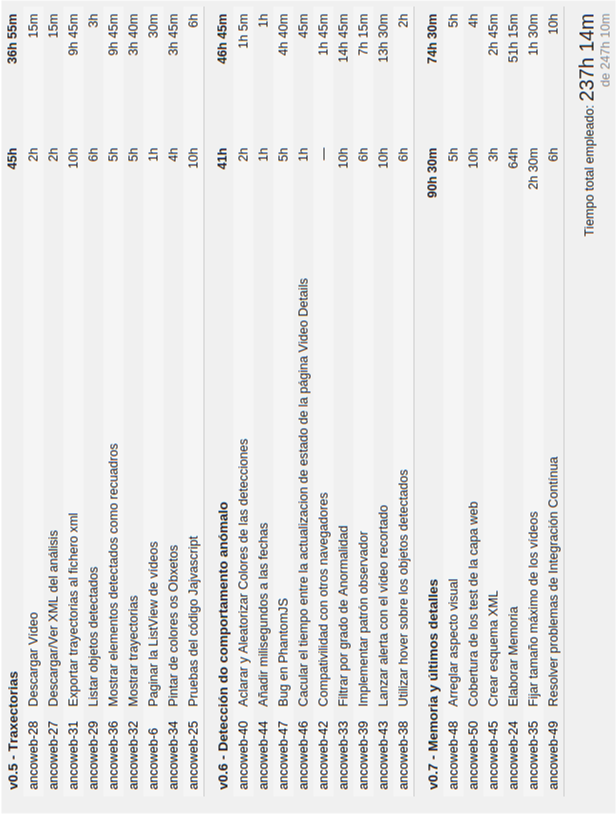
\includegraphics[scale=0.7]{figures/YouTrack/taboaHoras2_2.png}
    \caption{Táboa de horas adicadas ao proxecto por versión (2)}
\label{fig:taboaHoras2_2}
\end{center}
\end{figure}

Os datos do total de horas empregadas para a versión v1.0 suman 238 horas, que a un prezo de 
12 \euro a hora fan un custo total de 2.856,00 \euro.
